\section{Transform Coding and JPEG: The DCT Revolution}

\subsection{Learning Objectives}

By the end of this lecture, you will be able to:
\begin{enumerate}[leftmargin=*, nosep]
    \item Explain why transform coding is necessary for efficient lossy compression.
    \item Describe the energy-compaction property of the DCT and state why it approximates the optimal KL transform for natural images.
    \item Execute the complete JPEG pipeline on an $8\times8$ block: level-shift $\to$ 2D DCT $\to$ quantisation $\to$ zig-zag scan $\to$ RLE $\to$ Huffman.
    \item Quantify the rate–distortion trade-off controlled by the JPEG quality factor.
    \item Identify the physical cause of blocking, ringing, banding, and colour-bleeding artefacts.
    \item Connect JPEG's entropy-coding stage to Huffman coding and RLE from earlier lectures.
\end{enumerate}

\subsection{Motivation: Why Transform Coding?}

\subsubsection{Spatial Redundancy in Natural Images}

Raw pixel values in natural images are \emph{highly correlated}: a pixel is almost always very similar to its neighbours. Table~\ref{tab:rawblock} shows a representative $8\times8$ luminance block taken from a photograph of a clear sky.

\begin{table}[H]
\centering
\caption{Raw $8\times8$ luminance block (pixel values 0–255). Slow spatial variation is evident.}
\label{tab:rawblock}
\setlength{\tabcolsep}{5pt}
\begin{tabular}{|c|c|c|c|c|c|c|c|}
\hline
\rowcolor{LightBlue!20}
142 & 148 & 155 & 160 & 158 & 150 & 145 & 140 \\
\hline
140 & 146 & 153 & 158 & 156 & 148 & 143 & 138 \\
\hline
\rowcolor{LightGray!10}
138 & 144 & 151 & 156 & 154 & 146 & 141 & 136 \\
\hline
135 & 141 & 148 & 153 & 151 & 143 & 138 & 133 \\
\hline
\rowcolor{LightGray!10}
132 & 138 & 145 & 150 & 148 & 140 & 135 & 130 \\
\hline
130 & 136 & 143 & 148 & 146 & 138 & 133 & 128 \\
\hline
\rowcolor{LightGray!10}
128 & 134 & 141 & 146 & 144 & 136 & 131 & 126 \\
\hline
125 & 131 & 138 & 143 & 141 & 133 & 128 & 123 \\
\hline
\end{tabular}
\end{table}

\begin{importantbox}
\textbf{The Core Problem:} Huffman coding assigns short codes to \emph{frequent symbols}. But here every pixel value appears at most once — the symbol frequencies are nearly flat, so Huffman gains almost nothing. The redundancy is \emph{structural}, encoded in smooth spatial transitions, not in symbol repetition. We need a different representation to expose it.
\end{importantbox}

\subsubsection{The Transform-Coding Idea}

\begin{definitionbox}
\textbf{Transform Coding:} Apply a reversible linear transform $T$ to convert a block of $N$ correlated samples into $N$ \textbf{decorrelated coefficients} such that most of the signal energy concentrates into a small number of coefficients. The transform itself is \emph{lossless}; loss is introduced later, during quantisation.
\end{definitionbox}

The conceptual chain is:

\vspace{6pt}
\begin{center}
\begin{tikzpicture}[
    node distance = 1.2cm,
    box/.style = {
        draw,
        rounded corners=4pt,
        minimum width=2.6cm,
        minimum height=0.9cm,
        align=center,
        font=\small,
        text=black,
        fill opacity=1
    },
    lossless/.style = {box, fill=blue!15, draw=blue!70!black},
    lossy/.style    = {box, fill=red!15,  draw=red!70!black},
    arr/.style      = {-{Stealth[length=5pt]}, thick}
  ]

  \node[lossless] (T) {Transform\\(DCT)};
  \node[lossy, right=of T] (Q) {Quantisation};
  \node[lossless, right=of Q] (E) {Entropy\\Coding};

  \draw[arr] (T) -- (Q);
  \draw[arr] (Q) -- (E);

  \node[below=0.2cm of T, font=\scriptsize\itshape, text=blue!70!black] {lossless};
  \node[below=0.2cm of Q, font=\scriptsize\bfseries, text=red!70!black] {LOSSY};
  \node[below=0.2cm of E, font=\scriptsize\itshape, text=blue!70!black] {lossless};

\end{tikzpicture}
\end{center}
\vspace{4pt}

This three-stage structure is \textbf{universal}: JPEG (images), MP3/AAC (audio), H.264/H.265 (video), and HEIC all follow it.

\subsection{The Discrete Cosine Transform}

\subsubsection{Intuition: Change of Basis}

Any $8\times8$ image block $p(x,y)$ can be written as a weighted sum of 64 fixed $8\times8$ \textbf{basis patterns} $B_{u,v}(x,y)$:
\[
p(x,y) = \sum_{u=0}^{7}\sum_{v=0}^{7} D(u,v)\,B_{u,v}(x,y).
\]
The coefficients $D(u,v)$ are the \emph{coordinates} of the block in the DCT basis.

\begin{figure}[H]
\centering
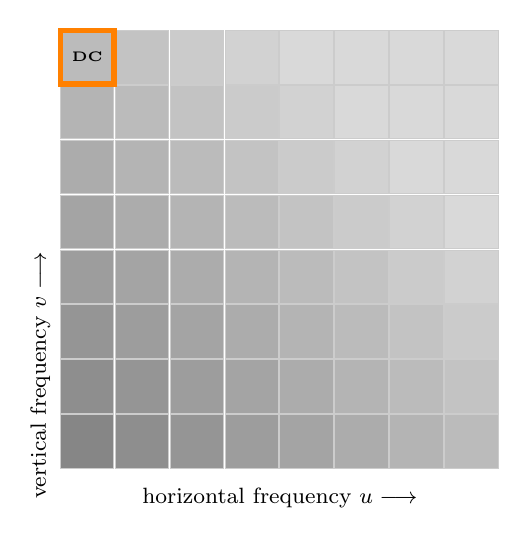
\begin{tikzpicture}[scale=0.85]
  % 8x8 grid with brightness decreasing toward bottom-right
  \foreach \u in {0,...,7}{
    \foreach \v in {0,...,7}{
      \pgfmathtruncatemacro{\bval}{95 - (\u+\v)*6}
      \pgfmathtruncatemacro{\bval}{max(\bval,30)}  % Minimum 30% to keep text visible
      \fill[gray!\bval!white] (\u*0.82, \v*0.82) rectangle ++(0.80,0.80);
      \draw[gray!40, line width=0.3pt] (\u*0.82, \v*0.82) rectangle ++(0.80,0.80);
    }
  }
  % Highlight DC cell with orange border
  \draw[orange, line width=2pt] (0,7*0.82) rectangle ++(0.80,0.80);
  \node[font=\tiny\bfseries, text=black] at (0.40, 7*0.82+0.40) {DC};
  % Add frequency labels with white background for visibility
  \node[below, font=\footnotesize, fill=white, fill opacity=0.7, text opacity=1, inner sep=1pt] at (3.28,-0.25) {horizontal frequency $u \longrightarrow$};
  \node[left, rotate=90, font=\footnotesize, fill=white, fill opacity=0.7, text opacity=1, inner sep=1pt] at (-0.3, 3.28) {vertical frequency $v \longrightarrow$};
\end{tikzpicture}
\caption{Schematic of the 64 DCT basis functions for an $8\times8$ block. The top-left cell (orange border) is the \textbf{DC} basis — a uniform block representing average brightness. Moving right increases horizontal frequency; moving down increases vertical frequency. Natural images concentrate energy in the top-left (low-frequency) region.}
\label{fig:basis}
\end{figure}

\subsubsection{The 2D DCT Formula}

\begin{definitionbox}
\textbf{2D DCT (Type-II):} For an $8\times8$ block $p(x,y)$, $x,y\in\{0,\ldots,7\}$:
\begin{equation}
\boxed{
  D(u,v) = \frac{C(u)\,C(v)}{4}
  \sum_{x=0}^{7}\sum_{y=0}^{7}
  p(x,y)\,
  \cos\!\left(\frac{(2x+1)\,u\,\pi}{16}\right)
  \cos\!\left(\frac{(2y+1)\,v\,\pi}{16}\right)
}
\label{eq:dct}
\end{equation}
where
\begin{equation}
  C(k) = \begin{cases} 1/\sqrt{2} & k=0, \\ 1 & k > 0. \end{cases}
\end{equation}
\end{definitionbox}

\paragraph{Inverse DCT (IDCT):} The transform is orthogonal, so the inverse uses the same cosine kernels with roles swapped:
\begin{equation}
  \hat{p}(x,y) = \frac{1}{4}
  \sum_{u=0}^{7}\sum_{v=0}^{7}
  C(u)\,C(v)\,D(u,v)\,
  \cos\!\left(\frac{(2x+1)\,u\,\pi}{16}\right)
  \cos\!\left(\frac{(2y+1)\,v\,\pi}{16}\right).
\label{eq:idct}
\end{equation}
After exact (unquantised) DCT$\to$IDCT, $\hat{p}=p$ to floating-point precision.

\subsubsection{Separability and Computational Cost}

Because the cosine kernel factorises as $\cos(\cdots u\cdots)\cos(\cdots v\cdots)$, the 2D DCT is \textbf{separable}:
\begin{equation}
  \text{2D-DCT} = \underbrace{\text{1D-DCT}_{\text{cols}}}_{\text{second pass}}
  \Bigl(\underbrace{\text{1D-DCT}_{\text{rows}}}_{\text{first pass}}(\mathbf{P})\Bigr).
\end{equation}

\begin{importantbox}
\textbf{Why Separability Matters:} Direct 2D summation in Eq.~\eqref{eq:dct} costs $O(N^4)$ multiplications for an $N\times N$ block. Separability reduces this to $O(N^3)$, and the fast DCT algorithm (analogous to the FFT) reduces it further to $O(N^2\log N)$. For $N=8$ this means 64 multiplications instead of 4096 — a 64$\times$ speedup.
\end{importantbox}

\subsubsection{Why DCT, Not DFT?}

The Discrete Fourier Transform (DFT) requires \emph{complex} coefficients and implicitly assumes the signal repeats periodically. Pixel blocks do not: abrupt discontinuities at block boundaries would introduce large high-frequency DFT coefficients, hurting compression. The DCT implicitly treats the block as if it were reflected (even-extended) at its boundaries, giving a much smoother periodic signal and therefore better energy compaction.

\begin{definitionbox}
\textbf{Why the DCT is (Nearly) Optimal:} The theoretically optimal linear decorrelating transform for a stationary signal is the \textbf{Karhunen--Lo\`eve Transform (KLT)}, which diagonalises the signal covariance matrix. For a first-order Markov model with correlation coefficient $\rho\to1$ (i.e., slowly varying signals, exactly the natural-image case), the KLT converges to the DCT. In practice, $\rho\approx0.97$ for typical images — the DCT is essentially optimal.
\end{definitionbox}

\subsection{Complete Pipeline: Step-by-Step Worked Example}

We now trace our example block through every stage of JPEG compression.

\subsubsection{Step 1 — Level Shift}

Subtract 128 from every pixel to centre the values around zero.

\begin{equation}
  p'(x,y) = p(x,y) - 128.
\end{equation}

\begin{table}[H]
\centering
\caption{Level-shifted block $p'(x,y)$. Positive values are in the upper-right, negative in the lower-left, consistent with the gentle brightness gradient in the original.}
\label{tab:levelshift}
\setlength{\tabcolsep}{5pt}
\begin{tabular}{|r|r|r|r|r|r|r|r|}
\hline
\rowcolor{LightBlue!40}
$+14$ & $+20$ & $+27$ & $+32$ & $+30$ & $+22$ & $+17$ & $+12$ \\
\hline
$+12$ & $+18$ & $+25$ & $+30$ & $+28$ & $+20$ & $+15$ & $+10$ \\
\hline
\rowcolor{LightGray}
$+10$ & $+16$ & $+23$ & $+28$ & $+26$ & $+18$ & $+13$ & $+8$  \\
\hline
$+7$  & $+13$ & $+20$ & $+25$ & $+23$ & $+15$ & $+10$ & $+5$  \\
\hline
\rowcolor{LightGray}
$+4$  & $+10$ & $+17$ & $+22$ & $+20$ & $+12$ & $+7$  & $+2$  \\
\hline
$+2$  & $+8$  & $+15$ & $+20$ & $+18$ & $+10$ & $+5$  & $0$   \\
\hline
\rowcolor{LightGray}
$0$   & $+6$  & $+13$ & $+18$ & $+16$ & $+8$  & $+3$  & $-2$  \\
\hline
$-3$  & $+3$  & $+10$ & $+15$ & $+13$ & $+5$  & $0$   & $-5$  \\
\hline
\end{tabular}
\end{table}

\subsubsection{Step 2 — Apply the 2D DCT}

Apply the 1D DCT to each row, then each column. The result is the coefficient matrix in Table~\ref{tab:dct}.

\begin{table}[H]
\centering
\caption{2D DCT coefficient matrix $D(u,v)$. The DC term dominates. Only the top-left $3\times3$ region contains non-negligible values.}
\label{tab:dct}
\setlength{\tabcolsep}{4pt}
\begin{tabular}{|r|r|r|r|r|r|r|r|}
\hline
\cellcolor{DCColor}\textbf{950} & \cellcolor{ACColor}$-12$ &
  \cellcolor{ACColor}$+3$ & $-2$ & $+1$ & $-1$ & $0$ & $0$ \\
\hline
\cellcolor{ACColor}$-15$ & \cellcolor{ACColor}$+8$ & $-4$ &
  $+2$ & $-1$ & $0$ & $0$ & $0$ \\
\hline
$+5$ & $-3$ & $+2$ & $-1$ & $0$ & $0$ & $0$ & $0$ \\
\hline
$-2$ & $+1$ & $-1$ & $0$ & $0$ & $0$ & $0$ & $0$ \\
\hline
$+1$ & $-1$ & $0$ & $0$ & $0$ & $0$ & $0$ & $0$ \\
\hline
$0$ & $0$ & $0$ & $0$ & $0$ & $0$ & $0$ & $0$ \\
\hline
$0$ & $0$ & $0$ & $0$ & $0$ & $0$ & $0$ & $0$ \\
\hline
$0$ & $0$ & $0$ & $0$ & $0$ & $0$ & $0$ & $0$ \\
\hline
\end{tabular}

\vspace{4pt}
{\small\color{MedGray}
  \textcolor{DCColor!80!black}{\rule{10pt}{8pt}} DC coefficient \quad
  \textcolor{ACColor!80!black}{\rule{10pt}{8pt}} significant AC coefficients \quad
  white = negligible}
\end{table}

\begin{examplebox}
\textbf{Verifying $D(0,0)$:} $D(0,0)$ equals the block mean scaled by $N=8$:
\[
  D(0,0) = \frac{C(0)^2}{4}\sum_{x,y} p'(x,y)
  = \frac{(1/\sqrt{2})^2}{4}\cdot \underbrace{\sum_{x,y} p'(x,y)}_{=\text{sum of all level-shifted values}}
  = \frac{1}{8}\cdot\text{(sum)}.
\]
The sum of the 64 level-shifted values in Table~\ref{tab:levelshift} is approximately $7600$, giving $D(0,0)\approx 7600/8 = 950$.
\end{examplebox}

\begin{importantbox}
\textbf{Energy Compaction — the ``Aha!'' Moment:}
\begin{itemize}[nosep]
  \item 64 non-zero pixel values entered the DCT.
  \item Only \textbf{approximately 12 non-zero} coefficients came out.
  \item $|D(0,0)|=950$ holds approximately $98\%$ of the signal energy.
  \item Coefficients beyond the top-left $3\times3$ corner are zero or negligible.
\end{itemize}
This is the energy-compaction property. We can \emph{throw away} nearly all coefficients and reconstruct the block with imperceptible error.
\end{importantbox}

\subsubsection{Step 3 — Quantisation}

\begin{definitionbox}
\textbf{Scalar Quantisation:} Each coefficient $D(u,v)$ is divided by a quantisation step $Q(u,v)$ and rounded:
\begin{equation}
  \hat{D}(u,v) = \operatorname{round}\!\left(\frac{D(u,v)}{Q(u,v)}\right).
\end{equation}
This is the \textbf{only irreversible step} in the entire JPEG pipeline.
\end{definitionbox}

\begin{table}[H]
\centering
\caption{JPEG standard luminance quantisation table at quality~50. Highlighted: \colorbox{LightGreen}{small steps} (low frequency) and \colorbox{LightRed}{large steps} (high frequency).}
\label{tab:qtable}
\setlength{\tabcolsep}{5pt}
\begin{tabular}{|c|c|c|c|c|c|c|c|}
\hline
\cellcolor{LightGreen}16 & \cellcolor{LightGreen}11 & \cellcolor{LightGreen}10 &
  16 & 24 & 40 & \cellcolor{LightRed}51 & \cellcolor{LightRed}61 \\
\hline
\cellcolor{LightGreen}12 & \cellcolor{LightGreen}12 & 14 & 19 & 26 &
  \cellcolor{LightRed}58 & \cellcolor{LightRed}60 & \cellcolor{LightRed}55 \\
\hline
14 & 13 & 16 & 24 & 40 & \cellcolor{LightRed}57 & \cellcolor{LightRed}69 &
  \cellcolor{LightRed}56 \\
\hline
14 & 17 & 22 & 29 & \cellcolor{LightRed}51 & \cellcolor{LightRed}87 &
  \cellcolor{LightRed}80 & \cellcolor{LightRed}62 \\
\hline
18 & 22 & 37 & \cellcolor{LightRed}56 & \cellcolor{LightRed}68 &
  \cellcolor{LightRed}109 & \cellcolor{LightRed}103 & \cellcolor{LightRed}77 \\
\hline
24 & 35 & \cellcolor{LightRed}55 & \cellcolor{LightRed}64 & \cellcolor{LightRed}81 &
  \cellcolor{LightRed}104 & \cellcolor{LightRed}113 & \cellcolor{LightRed}92 \\
\hline
\cellcolor{LightRed}49 & \cellcolor{LightRed}64 & \cellcolor{LightRed}78 &
  \cellcolor{LightRed}87 & \cellcolor{LightRed}103 & \cellcolor{LightRed}121 &
  \cellcolor{LightRed}120 & \cellcolor{LightRed}101 \\
\hline
\cellcolor{LightRed}72 & \cellcolor{LightRed}92 & \cellcolor{LightRed}95 &
  \cellcolor{LightRed}98 & \cellcolor{LightRed}112 & \cellcolor{LightRed}100 &
  \cellcolor{LightRed}103 & \cellcolor{LightRed}99 \\
\hline
\end{tabular}
\end{table}

\begin{examplebox}
\textbf{Quantisation at Quality 50:}
\[
  \hat{D}(0,0) = \operatorname{round}\!\left(\frac{950}{16}\right) = \operatorname{round}(59.375) = \mathbf{59}
\]
\[
  \hat{D}(0,1) = \operatorname{round}\!\left(\frac{-12}{11}\right) = \operatorname{round}(-1.09) = \mathbf{-1}
\]
\[
  \hat{D}(1,0) = \operatorname{round}\!\left(\frac{-15}{12}\right) = \operatorname{round}(-1.25) = \mathbf{-1}
\]
\[
  \hat{D}(0,2) = \operatorname{round}\!\left(\frac{3}{10}\right) = \operatorname{round}(0.30) = \mathbf{0} \;\;\text{(discarded!)}
\]
\end{examplebox}

The full quantised coefficient matrix:

\begin{table}[H]
\centering
\caption{Quantised DCT coefficients $\hat{D}(u,v)$ at quality~50. Only 3 non-zero values survive from the original 64.}
\label{tab:quantcoeffs}
\setlength{\tabcolsep}{5pt}
\begin{tabular}{|r|r|r|r|r|r|r|r|}
\hline
\cellcolor{DCColor}\textbf{59} & \cellcolor{LightRed}$-1$ & $0$ & $0$ & $0$ & $0$ & $0$ & $0$ \\
\hline
\cellcolor{LightRed}$-1$ & $0$ & $0$ & $0$ & $0$ & $0$ & $0$ & $0$ \\
\hline
$0$ & $0$ & $0$ & $0$ & $0$ & $0$ & $0$ & $0$ \\
\hline
$0$ & $0$ & $0$ & $0$ & $0$ & $0$ & $0$ & $0$ \\
\hline
$0$ & $0$ & $0$ & $0$ & $0$ & $0$ & $0$ & $0$ \\
\hline
$0$ & $0$ & $0$ & $0$ & $0$ & $0$ & $0$ & $0$ \\
\hline
$0$ & $0$ & $0$ & $0$ & $0$ & $0$ & $0$ & $0$ \\
\hline
$0$ & $0$ & $0$ & $0$ & $0$ & $0$ & $0$ & $0$ \\
\hline
\end{tabular}
\end{table}

\begin{warningbox}
\textbf{Irreversibility of Quantisation:} The decoder performs \emph{inverse quantisation} by multiplying: $\tilde{D}(u,v)=\hat{D}(u,v)\cdot Q(u,v)$. For the DC term: $59\times16=944\neq950$. The error of 6 units is permanent. The IDCT then spreads this error across all 64 reconstructed pixels — this manifests as the subtle tonal shift we perceive at low quality factors.
\end{warningbox}

\subsubsection{Step 4 — Zig-Zag Scan}

The quantised $8\times8$ matrix is serialised into a 1D sequence by traversing in zig-zag order.

\begin{figure}[H]
\centering
\begin{tikzpicture}[scale=0.72]
  % Draw the 8x8 grid with light gray lines
  \foreach \i in {0,...,7}
    \foreach \j in {0,...,7}
      \draw[gray!40, line width=0.5pt] (\i,\j) rectangle ++(1,1);

  % Highlight DC cell with yellow fill and orange border
  \fill[DCColor] (0,7) rectangle (1,8);
  \draw[orange, line width=2pt] (0,7) rectangle (1,8);
  \node[font=\tiny\bfseries, text=black] at (0.5,7.5) {DC};

  % Draw zigzag path with arrows using blue!75!black
  \draw[blue!75!black, thick, -{Stealth[length=5pt]}] 
    (0.5,7.5) -- (1.5,7.5) -- (1.5,6.5) -- (0.5,6.5) -- 
    (0.5,5.5) -- (1.5,5.5) -- (2.5,5.5) -- (2.5,6.5) -- 
    (2.5,7.5) -- (3.5,7.5) -- (4.5,7.5) -- (4.5,6.5) -- 
    (3.5,6.5) -- (3.5,5.5) -- (3.5,4.5) -- (2.5,4.5) -- 
    (1.5,4.5) -- (0.5,4.5);

  % Labels with white background for visibility
  \node[below, font=\footnotesize, fill=white, fill opacity=0.7, text opacity=1, inner sep=2pt] at (4,0) {$u$ (horizontal freq.) $\longrightarrow$};
  \node[left, rotate=90, font=\footnotesize, fill=white, fill opacity=0.7, text opacity=1, inner sep=2pt] at (-0.5,4) {$\longleftarrow$ $v$ (vertical freq.)};
  
  % Start marker
  \node[font=\tiny, fill=white, fill opacity=0.7, text opacity=1, inner sep=1pt] at (0.5,8.2) {Start};
\end{tikzpicture}
\caption{\textbf{Zig-zag scan order} on the $8\times8$ quantised coefficient matrix. The path begins at DC (top-left) and sweeps toward high frequencies (bottom-right), ensuring that the long run of trailing zeros appears at the \emph{end} of the 1D sequence.}
\label{fig:zigzag}
\end{figure}

Applying zig-zag to our quantised matrix in Table~\ref{tab:quantcoeffs}:
\[
\underbrace{59}_{\text{DC}},\;
\underbrace{-1,\;-1}_{\text{2 AC non-zeros}},\;
\underbrace{0,\;0,\;\ldots,\;0}_{61\text{ zeros}}.
\]

\subsubsection{Step 5 — Run-Length Encoding (RLE)}

\begin{definitionbox}
\textbf{JPEG AC RLE Format:} Each non-zero AC coefficient is encoded as a pair \texttt{(RUNLENGTH, VALUE)} where \texttt{RUNLENGTH} is the count of zero coefficients immediately preceding it (0--15). A special \textbf{End-of-Block (EOB)} symbol \texttt{(0,0)} signals that all remaining coefficients in the block are zero.
\end{definitionbox}

For our example sequence $[59,\,-1,\,-1,\,\underbrace{0,\ldots,0}_{61}]$:

\begin{center}
\begin{tabular}{lll}
\toprule
\textbf{Symbol} & \textbf{Meaning} & \textbf{Value} \\
\midrule
DC (DPCM) & difference from previous block's DC & $59 - \text{prev}$ \\
\texttt{(0,\;$-1$)} & 0 zeros before, AC value $= -1$ & \\
\texttt{(0,\;$-1$)} & 0 zeros before, AC value $= -1$ & \\
\texttt{EOB} & all remaining 61 coefficients are 0 & \\
\bottomrule
\end{tabular}
\end{center}

\begin{importantbox}
\textbf{Why DPCM for DC?} Adjacent $8\times8$ blocks in a natural image share similar average brightness, so their DC coefficients differ by small amounts. Encoding the \emph{difference} (DPCM) produces small values with a narrow histogram — perfect for Huffman coding. AC coefficients do not have this cross-block regularity, so DPCM is not applied to them.
\end{importantbox}

\subsubsection{Step 6 — Huffman Coding}

JPEG uses pre-defined Huffman tables (stored in the file header) separately for DC and AC symbols. Each symbol comprises two parts:

\begin{enumerate}[nosep]
  \item \textbf{Huffman code:} encodes the \emph{category} $k$ where $|x|\in[2^{k-1},2^k-1]$ for a coefficient value $x$.
  \item \textbf{Additional bits:} $k$ raw bits that identify the exact value within the category (for $k=0$ only the EOB symbol, no extra bits).
\end{enumerate}

\begin{examplebox}
\textbf{Huffman Encoding of $\hat{D}(0,0)=59$:} DC difference $= 59$. Category: $k=6$ since $2^5=32 \le 59 < 64=2^6$. The value $59$ is encoded as the category-6 Huffman code (variable length, typically approximately 4 bits from JPEG tables) followed by 6 additional bits representing $59$ in offset-binary. Total approximately 10 bits for the DC term.
\end{examplebox}

\begin{connectionbox}
\textbf{Connections to Previous Lectures:}
\begin{itemize}[nosep]
  \item \textbf{Lecture 3 (Huffman):} JPEG uses the same prefix-free code construction but with fixed, pre-optimised tables rather than image-adaptive ones.
  \item \textbf{Lecture 7 (RLE):} The (RUNLENGTH, VALUE) pairs directly implement the run-length encoding discussed for 1D sequences.
  \item \textbf{Lecture 6 (DEFLATE):} DEFLATE also combines LZ77 (run-length style) with Huffman; JPEG's entropy stage is a specialised version tailored to DCT coefficient statistics.
\end{itemize}
\end{connectionbox}

\subsection{Complete JPEG Encoder and Decoder}

\subsubsection{Colour Pre-Processing}

Colour JPEG images are first converted from RGB to \textbf{YC\textsubscript{b}C\textsubscript{r}}:

\begin{align}
  Y  &= 0.299R + 0.587G + 0.114B \tag{luminance}\\
  C_b &= 128 - 0.168736R - 0.331264G + 0.5B \tag{blue chroma}\\
  C_r &= 128 + 0.5R - 0.418688G - 0.081312B \tag{red chroma}
\end{align}

The human visual system resolves luminance at roughly $4\times$ the spatial acuity of chrominance. JPEG exploits this by \textbf{4:2:0 chroma subsampling}: each $2\times2$ block of luma pixels shares a single $C_b$ and $C_r$ value. This alone achieves a 2:1 reduction in chroma data with negligible perceptual impact.

\subsubsection{Block Diagram}

\begin{figure}[H]
\centering
\begin{tikzpicture}[
    node distance = 0.45cm and 0.3cm,
    block/.style  = {draw, rounded corners=4pt, minimum width=1.6cm,
                     minimum height=0.7cm, align=center, font=\scriptsize},
    preproc/.style= {block, fill=LightBlue!70,   draw=blue!75!black},
    dctb/.style   = {block, fill=LightOrange!70, draw=orange!75!black},
    lossy/.style  = {block, fill=LightRed!70,    draw=red!75!black},
    entb/.style   = {block, fill=LightGreen!70,  draw=green!50!black},
    arr/.style    = {-{Stealth[length=4pt]}, thick, color=black!60}
  ]
  \node[preproc] (rgb)  {RGB $\to$\\YCbCr};
  \node[preproc, right=of rgb]  (sub)  {4:2:0\\Subsampling};
  \node[preproc, right=of sub]  (blk)  {Split\\8$\times$8};
  \node[preproc, right=of blk]  (lvl)  {Level\\shift};
  \node[dctb,   right=of lvl]   (dct)  {2D\\DCT};
  \node[lossy,  right=of dct]   (qnt)  {Quant\-ise};
  \node[entb,   right=of qnt]   (zz)   {Zig-\\Zag};
  \node[entb,   right=of zz]    (rle)  {RLE\\DPCM};
  \node[entb,   right=of rle]   (huf)  {Huffman};

  \foreach \a/\b in {rgb/sub,sub/blk,blk/lvl,lvl/dct,dct/qnt,qnt/zz,zz/rle,rle/huf}
    \draw[arr] (\a)--(\b);

  \node[above=0.35cm of rgb, font=\tiny, color=blue!75!black]  {colour};
  \node[above=0.35cm of dct, font=\tiny, color=orange!75!black]{transform};
  \node[above=0.35cm of qnt, font=\tiny\bfseries, color=red!75!black]  {LOSSY};
  \node[above=0.35cm of huf, font=\tiny, color=green!50!black] {entropy};
\end{tikzpicture}
\caption{Complete JPEG encoding pipeline. The three inner stages (DCT, Quantise, Entropy) handle each $8\times8$ block independently; the colour stages process the whole image once at the start.}
\label{fig:pipeline}
\end{figure}

\subsubsection{Decoding Is the Exact Reverse}

\begin{center}
\begin{tikzpicture}[
    node distance = 0.45cm and 0.3cm,
    block/.style  = {draw, rounded corners=4pt, minimum width=1.7cm,
                     minimum height=0.7cm, align=center, font=\scriptsize},
    entb/.style   = {block, fill=LightGreen!70,  draw=green!50!black},
    dctb/.style   = {block, fill=LightOrange!70, draw=orange!75!black},
    iqb/.style    = {block, fill=LightRed!40,    draw=red!75!black},
    postb/.style  = {block, fill=LightBlue!70,   draw=blue!75!black},
    arr/.style    = {-{Stealth[length=4pt]}, thick, color=black!60}
  ]
  \node[entb]  (huf) {Huffman\\decode};
  \node[entb,  right=of huf] (rle) {RLE\\decode};
  \node[entb,  right=of rle] (izz) {Inv.\\Zig-Zag};
  \node[iqb,   right=of izz] (iq)  {Inv.\\Quantise};
  \node[dctb,  right=of iq]  (idt) {IDCT};
  \node[postb, right=of idt] (add) {$+128$};
  \node[postb, right=of add] (up)  {4:2:0\\Upsample};
  \node[postb, right=of up]  (rgb) {YCbCr\\$\to$ RGB};

  \foreach \a/\b in {huf/rle,rle/izz,izz/iq,iq/idt,idt/add,add/up,up/rgb}
    \draw[arr] (\a)--(\b);

  \node[above=0.35cm of iq, font=\tiny, color=red!75!black] {\textit{approx. only}};
\end{tikzpicture}
\end{center}

The inverse quantisation step is \emph{approximate}: $\tilde{D}(u,v)=\hat{D}(u,v)\cdot Q(u,v)$, which in general $\neq D(u,v)$ due to rounding during forward quantisation.

\subsection{Rate–Distortion Trade-off}

\subsubsection{The PSNR Metric}

Image quality after lossy compression is typically measured by \textbf{Peak Signal-to-Noise Ratio (PSNR)}:
\begin{equation}
  \mathrm{PSNR} = 10\log_{10}\!\left(\frac{255^2}{\mathrm{MSE}}\right)\;\text{dB},
  \qquad
  \mathrm{MSE} = \frac{1}{HW}\sum_{x,y}(p(x,y)-\hat{p}(x,y))^2.
\end{equation}
Higher PSNR = better quality; $>40$ dB is generally considered visually lossless for natural images.

\begin{figure}[H]
\centering
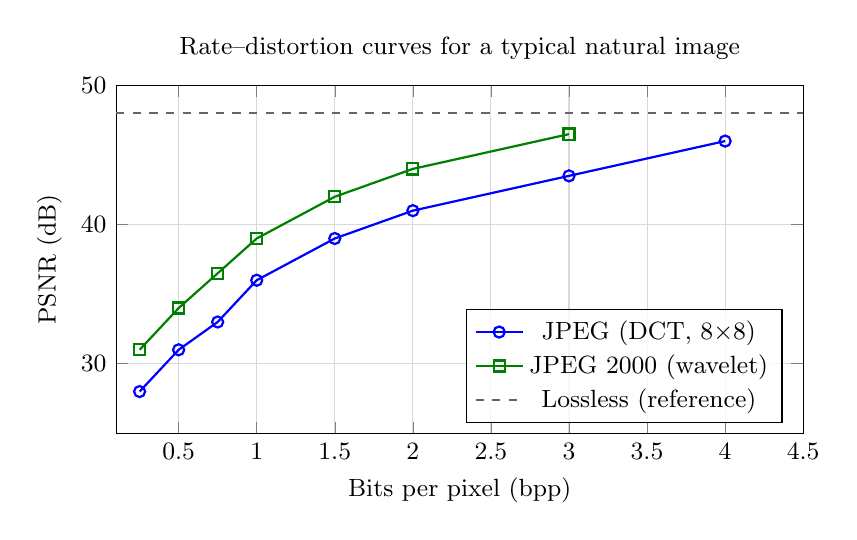
\begin{tikzpicture}
\begin{axis}[
  width=0.85\textwidth, height=6cm,
  xlabel={Bits per pixel (bpp)},
  ylabel={PSNR (dB)},
  xmin=0.1, xmax=4.5,
  ymin=25, ymax=50,
  grid=major, grid style={gray!30},
  legend pos=south east,
  legend style={font=\small, fill=white, fill opacity=0.8, text opacity=1},
  label style={font=\small},
  tick label style={font=\small},
  title={Rate–distortion curves for a typical natural image},
  title style={font=\small},
  every axis plot/.append style={thick},
]
% JPEG empirical values
\addplot[blue, mark=o, mark size=2pt] coordinates {
  (0.25,28) (0.50,31) (0.75,33) (1.0,36) (1.5,39) (2.0,41) (3.0,43.5) (4.0,46)
};
\addlegendentry{JPEG (DCT, 8$\times$8)}

% JPEG 2000
\addplot[green!50!black, mark=square, mark size=2pt] coordinates {
  (0.25,31) (0.50,34) (0.75,36.5) (1.0,39) (1.5,42) (2.0,44) (3.0,46.5)
};
\addlegendentry{JPEG 2000 (wavelet)}

% Lossless reference line
\addplot[black!60, dashed] coordinates {(0.1,48) (4.5,48)};
\addlegendentry{Lossless (reference)}
\end{axis}
\end{tikzpicture}
\caption{Typical rate–distortion curves. At any given bit-rate, JPEG 2000 (wavelet) outperforms JPEG, but JPEG remains competitive for bpp $>1$.}
\label{fig:rd}
\end{figure}

\subsection{Compression Artefacts}

\begin{definitionbox}
\textbf{Compression Artefact:} A visual distortion introduced by lossy compression that was not present in the original image and is not present in the scene being depicted.
\end{definitionbox}

\subsubsection{Blocking Artefacts}

\textbf{Cause:} Each $8\times8$ block is quantised independently. At low quality, large quantisation errors produce abrupt changes in reconstructed pixel values at block boundaries.

\textbf{Visual appearance:} A visible rectangular grid superimposed on smooth image regions. Most noticeable in flat areas such as skies and skin tones.

\begin{figure}[H]
\centering
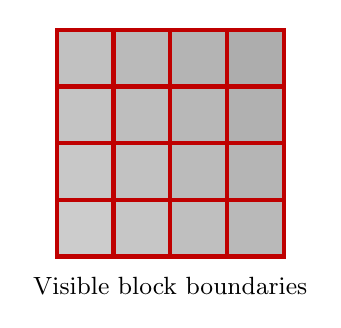
\begin{tikzpicture}[scale=0.6]
  % Simulate blocking artefact with distinct 8x8 blocks
  \foreach \i in {0,...,3} {
    \foreach \j in {0,...,3} {
      \pgfmathtruncatemacro{\shade}{40 + 5*\i + 3*\j}
      \fill[gray!\shade!white] (\i*1.2, \j*1.2) rectangle ++(1.2,1.2);
      \draw[red!75!black, line width=1.5pt] (\i*1.2, \j*1.2) rectangle ++(1.2,1.2);
    }
  }
  \node[below, font=\small, fill=white, fill opacity=0.7, text opacity=1, inner sep=2pt] at (2.4,-0.3) {Visible block boundaries};
\end{tikzpicture}
\caption{Blocking artefact — visible grid lines at $8\times8$ block boundaries.}
\label{fig:blocking}
\end{figure}

\subsubsection{Ringing Artefacts (Gibbs Phenomenon)}

\textbf{Cause:} Truncating high-frequency DCT coefficients is equivalent to multiplying the frequency-domain representation by a rectangular window. By the convolution theorem, this convolves the spatial image with a sinc-like kernel, producing oscillatory ringing near sharp edges.

\textbf{Visual appearance:} Faint light/dark halos around high-contrast edges (e.g., text on a coloured background, tree silhouettes against sky).

\begin{figure}[H]
\centering
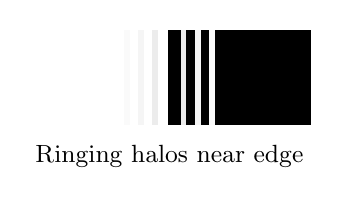
\begin{tikzpicture}[scale=0.6]
  % Sharp edge
  \fill[white] (0,0) rectangle (3,2);
  \fill[black] (3,0) rectangle (6,2);
  \draw[thick] (3,0) -- (3,2);
  
  % Ringing oscillations (sinc-like ripples)
  \draw[gray!15, line width=2pt] (2.7,0) -- (2.7,2);
  \draw[gray!8, line width=2pt] (2.4,0) -- (2.4,2);
  \draw[gray!4, line width=2pt] (2.1,0) -- (2.1,2);
  \draw[gray!15, line width=2pt] (3.3,0) -- (3.3,2);
  \draw[gray!8, line width=2pt] (3.6,0) -- (3.6,2);
  \draw[gray!4, line width=2pt] (3.9,0) -- (3.9,2);
  
  \node[below, font=\small, fill=white, fill opacity=0.7, text opacity=1, inner sep=2pt] at (3,-0.3) {Ringing halos near edge};
\end{tikzpicture}
\caption{Ringing artefact — oscillatory halos near a sharp black/white edge.}
\label{fig:ringing}
\end{figure}

\subsubsection{Banding / Posterisation}

\textbf{Cause:} Coarse quantisation of the DC coefficient and the lowest AC coefficients cannot represent the full tonal range of smooth gradients. The reconstructed image can only take on discrete levels spaced $Q(u,v)$ apart.

\textbf{Visual appearance:} Smooth gradients (blue sky, skin) appear as distinct bands of uniform tone rather than continuous variation.

\subsubsection{Colour Bleeding}

\textbf{Cause:} 4:2:0 chroma subsampling assigns a single $C_b/C_r$ value to each $2\times2$ luma block. At luminance edges, the chroma value may belong to the wrong side of the edge.

\textbf{Visual appearance:} Colour "bleeds" across sharp edges; particularly visible on coloured text or saturated objects.

\subsection{JPEG vs. Modern Formats}

\begin{table}[H]
\centering
\caption{Comparison of major lossy image compression standards (2024).}
\label{tab:formats}
\begin{tabular}{lccccccc}
\toprule
\textbf{Format} & \textbf{Year} & \textbf{Transform} &
  \textbf{Max block} & \textbf{Transparency} & \textbf{Animation} &
  \textbf{Royalty-free} \\
\midrule
JPEG         & 1992 & DCT    & $8\times8$    & No  & No  & Yes \\
JPEG 2000    & 2000 & Wavelet & Variable    & Yes & No  & Yes \\
WebP         & 2010 & DCT (VP8) & $16\times16$ & Yes & Yes & Yes \\
HEIC/HEIF    & 2017 & H.265 DCT & $64\times64$ & Yes & Yes & Contested \\
AVIF         & 2019 & AV1 DCT & $64\times64$ & Yes & Yes & Yes \\
\bottomrule
\end{tabular}
\end{table}

Despite modern formats offering better compression at equal quality, JPEG retains dominant market share because of three decades of universal toolchain support.

\subsection{When to Use (and Not Use) JPEG}

\begin{minipage}[t]{0.48\linewidth}
\begin{tcolorbox}[base, colback=LightGreen, colframe=green!50!black,
                  title={\textbf{Use JPEG for}}]
\begin{itemize}[nosep, leftmargin=*]
  \item Photographs and natural images
  \item Web delivery (universal support)
  \item Camera output / archival when space is limited
  \item Any image where approximately 5\% quality loss is acceptable
\end{itemize}
\end{tcolorbox}
\end{minipage}\hfill
\begin{minipage}[t]{0.48\linewidth}
\begin{tcolorbox}[base, colback=LightRed, colframe=red!75!black,
                  title={\textbf{Avoid JPEG for}}]
\begin{itemize}[nosep, leftmargin=*]
  \item Text, diagrams, line art (use PNG)
  \item Images needing transparency (use PNG/WebP)
  \item Medical / scientific images (use lossless)
  \item Files that will be re-edited and re-saved (generation loss!)
  \item Screenshots and UI graphics (use PNG)
\end{itemize}
\end{tcolorbox}
\end{minipage}

\vspace{10pt}

\begin{warningbox}
\textbf{Generation Loss:} Each JPEG save re-quantises the DCT coefficients. Saving a JPEG as JPEG ten times compounds quantisation error. After ten re-saves at quality~80, blocking and ringing artefacts that were invisible after one save become clearly visible. \textbf{Always edit in a lossless format; export to JPEG only as the final step.}
\end{warningbox}

\subsection{Summary}

\begin{importantbox}
\textbf{Five Key Insights of Transform Coding:}
\begin{enumerate}[nosep]
  \item \textbf{Decorrelation:} The DCT transforms spatially correlated pixels into (approximately) uncorrelated frequency coefficients.
  \item \textbf{Energy compaction:} Natural image energy concentrates in a small fraction of DCT coefficients (typically the top-left corner of the $8\times8$ matrix), enabling aggressive but selective discarding.
  \item \textbf{Single lossy step:} Quantisation is the \emph{only} irreversible operation. Every other step — DCT, zig-zag, RLE, Huffman — is lossless and reversible.
  \item \textbf{Perceptual exploitation:} The non-uniform Q-table encodes the human visual system's reduced sensitivity to high-frequency detail. We discard exactly what we cannot see.
  \item \textbf{Universality:} The transform $\to$ quantise $\to$ entropy-code paradigm extends directly to audio (MDCT in MP3/AAC), video (block DCT in H.264), and even speech coding.
\end{enumerate}
\end{importantbox}

\subsection{Exercises}

\begin{exercisebox}
\textbf{(DC coefficient)} Compute $D(0,0)$ for a uniform $8\times8$ block where every pixel equals 200. Show that $D(0,0) = 8\,\bar{p}'$ where $\bar{p}'$ is the mean of the level-shifted block. What does $D(0,0)=0$ imply about a block whose average brightness is exactly 128?
\end{exercisebox}

\begin{exercisebox}
\textbf{(Quantisation error)} A DCT coefficient $D(1,0)=-15$ is quantised with step $Q(1,0)=12$.
\begin{enumerate}[nosep, label=(\alph*)]
  \item Compute the quantised value $\hat{D}(1,0)$.
  \item Compute the reconstructed value $\tilde{D}(1,0) = \hat{D}(1,0)\times Q(1,0)$.
  \item Compute the absolute quantisation error.
\end{enumerate}
\end{exercisebox}

\begin{exercisebox}
\textbf{(Zig-zag and RLE)} A quantised $8\times8$ block has non-zero coefficients \emph{only} at positions $(0,0)=10$, $(2,0)=3$, $(0,2)=-2$. All others are zero.
\begin{enumerate}[nosep, label=(\alph*)]
  \item Write out the first 10 elements of the zig-zag sequence.
  \item Write the JPEG RLE encoding (DC treated separately).
\end{enumerate}
\end{exercisebox}

\begin{exercisebox}
\textbf{(Medical imaging)} A hospital proposes saving CT scans as JPEG at quality~80 to reduce storage costs. Identify two specific diagnostic risks, explain their technical cause using concepts from this lecture, and propose an alternative compression strategy that reduces storage without those risks.
\end{exercisebox}
